%&pdflatex
\documentclass[11pt]{article}

\usepackage{geometry}                % See geometry.pdf to learn the layout options. There are lots.
\usepackage{listings}
\usepackage{graphicx}
\geometry{letterpaper}                   % ... or a4paper or a5paper or ...

\usepackage{hyperref}
\usepackage{bookmark}

\setlength{\parindent}{0pt}
\setlength{\parskip}{\baselineskip}%

\title{Programming Applications (PRA) \\ Minor Coursework Exercise 4 \\
``Express(ions) yourself'' (2.5\%)}
%\author{Martin Chapman (martin.chapman@kcl.ac.uk)}
\date{}                                           % Activate to display a given date or no date

\begin{document}
\maketitle
%\section{}
%\subsection{}

%\vspace{-10mm}

\textbf{Please read the document marked `Q\&A Lab Projects and Pair Programming' carefully, before attempting any lab project. It contains important information on how to complete each minor piece of coursework, and is updated regularly. You will be asked to officially declare that you have read this document prior to submission. False declarations are taken seriously by both the department and by the college.}

\emph{This lab project counts for 2.5\% of your mark for PRA minor coursework assessment, and is the fourth of four.}

\emph{The release weeks for this assignment start 5th March, at 23:55, and end 19th March, at 23:55. All submissions must occur before the end of the second release week.}

\emph{If you have any questions about the structure of this assessment, please follow the `Additional Support' steps listed on KEATS.}

\textbf{You must select and work with a new partner for this piece of work}

The aims of the fourth lab project are as follows:

\begin{enumerate}
	
	\item To use regular expressions to solve practical problems;
	
	\item To continue working with components, layout managers and events.
	
\end{enumerate}

In the previous lab project, we introduced the hard constraint that, in your solution, classes representing the model and the view should not have any references to each other. This was a slightly unrealistic constraint, which was designed to encourage a critique of the model-view-controller design. In this lab project, we will introduce an additional (unrealistic) constraint, designed to encourage a critique of the applicability of regular expressions. This constraint is as follows: \textbf{no methods from the \texttt{String} class (or any other class that facilitates string manipulation) should be used during the construction of your solution to this assignment}, especially \texttt{replace}, \texttt{split} and \texttt{substring}. Note that this does \textbf{not} include \texttt{equals}, which originates from the \texttt{Object} class. Students who use methods from the \texttt{String} class will receive a maximum mark of 2 / 5 (40\%).

Note that your use of the MVC paradigm to structure your solution for this project is encouraged but not mandatory.

\section{Domain Description}
\label{sec:domain}

\emph{Media Servers}, in order to facilitate access to your personal media content, present a \emph{library} of available media. This library is often built from media source files that have heterogeneous naming schemes, yet the library itself is presented in a uniform manner. For example, the media source files shown in Figure \ref{fig:folder} have no consistent naming scheme, however the library shown in Figure \ref{fig:library} does, with pertinent information about each piece of media (e.g. its title, and an associated image) shown consistently for each item (note that the library in Figure \ref{fig:library} is not supposed to reflect the source content shown in Figure \ref{fig:folder}).

\begin{figure}[htbp]
\begin{center}
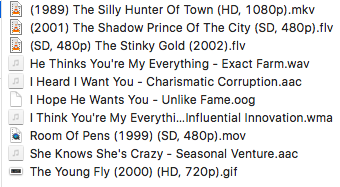
\includegraphics[width=300pt,height=160pt]{/Library/Server/Web/Data/Sites/webserver/PRA/distribute/CSnUsTh4/Assignment4Images/folder.png}
\caption{Raw media content from a file store.}
\label{fig:folder}
\end{center}
\end{figure}

\begin{figure}[htbp]
\begin{center}
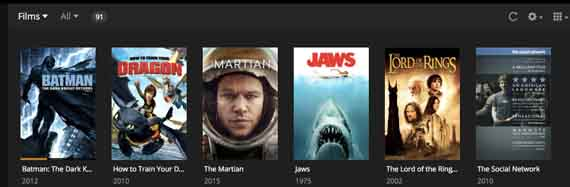
\includegraphics[width=460pt,height=150pt]{/Library/Server/Web/Data/Sites/webserver/PRA/distribute/CSnUsTh4/Assignment4Images/plex.jpg}
\caption{How a library on a Media Server may appear. In this example, we only have film media content, but media content may also include music.}
\label{fig:library}
\end{center}
\end{figure}

In this lab project, you will setup a library view for a media server.

\section{Setting up the packages}

Create a new \emph{project} in your chosen IDE. Inside this project, create a new \emph{package} named according to a concatenation of your first name, and the first name of your partner ($<$partnerApartnerB$>$). So, if Martin Chapman and Steffen Zschaler were embarking on this exercise, our project would contain a package called \emph{steffenmartin}. The order of names here is unimportant, but it is essential that you name your top-level package in this way, in order to identify your association with your partner to us.

If you locate the actual \emph{folder structure} created in your filesystem by your IDE for this project, you should now find an empty $<$\emph{partnerApartnerB}$>$ folder inside the source folder for your project. 

You should create additional packages for your project (perhaps for the model, view and controller), but this is not a strict requirement.

\subsection{Library Classes and Resources}

On KEATS you will find a package called \texttt{generator}. This package contains the source files required to generate a list of \emph{fictional} media file names, which we will use to test our library view, as opposed to data about real files. 

In order to generate this list, the \texttt{generator} package relies on a folder of \texttt{resources}. You will also find this folder on KEATS. The expected location for this folder is inside the IDE project folder you are using for the fourth minor piece of coursework, next to the \texttt{src} folder (i.e. in the location you would typically place files that are required for the running of a program, so that they can be accessed directly). 

Once the \texttt{resources} folder is in an accessible location, you can call the method \texttt{getMedia} from the class \texttt{generator.MediaGenerator} to obtain a list of the fictional file names that your library view will need to display. If, for some reason, you wish to change the location of the \texttt{resources} folder, you can specify a path to this folder using \texttt{getMedia( path )} (where this path should always end in \texttt{/resources}). In addition, if you are experiencing problems with loading data from the \texttt{resources} folder locally (via the \texttt{generator} package) you can instead instruct \texttt{MediaGenerator} to get this information from a remote location, using  \texttt{getMedia( true )}, although this will cause your program to load more slowly. Examine the source of \texttt{MediaGenerator} to understand both these parameters more closely.

Feel free to examine the remaining source of this code too (not all of it was developed especially for this project), but ensure that your solution \emph{only} relies the method \texttt{getMedia} inside \texttt{MediaGenerator}. \textbf{You should submit this package with your solution}, but solutions that are submitted with any of the files inside the \texttt{generator} package altered, will receive a mark of zero. The only exception to this is the alteration of the package names in each file, should you wish to include them in a particular place within your project.

\subsection{Source Data}

At this point, you should be able to call \texttt{getMedia} in your own program by importing \texttt{generator.MediaGenerator}, and then you should be able to print the list returned from this method to display output similar the following --

\texttt{[(HD, 720p) (1998) The Forever Pensioner Of The City.mpg, Saying It Like A Bird (2002) (SD, 480p).mkv, $\dots$]}

-- which is a \emph{sample} list, representing some of the file names your program will need to process. This objects in this list are of type \texttt{Media}, which has two fields: \texttt{name} and \texttt{image}. \texttt{MediaGenerator} uses images from the \texttt{resources} folder to combine each fictional media file name with fictional artwork associated with this piece of media, and packages them in a \texttt{Media} object. Real pieces of media artwork can be seen in Figure \ref{fig:library}. Examine the source of \texttt{Media} in order to learn more about how to access the data that instances of this class contain.

The names attributed to each \texttt{Media} object in this list have the following potential attributes:

\begin{itemize}

	\item They are either film or music (track) files. Film files have the extensions .flv, .gif, .mkv, .mpeg, .mpg or .mov., while track files have the extensions .aiff, .aac, .aax, .oog, .wav or .wma. Files of unknown type have no extension.
	
	\item The name of a film file contains the year the film was released, its quality and its title. The year of release (e.g. 1989) and the definition and pixels (e.g. HD, 720p) are placed in parenthesis, and either can feature anywhere inside the file name (i.e. either before or after the media name itself).
	
	\item The name of a track file contains the name of the track, followed by a hyphen (-) and then finally the name of the artist.
	
	\item Examine the source code inside \texttt{generator} to learn more about the potential file names you might encounter.

\end{itemize}

\subsection{Showing the library}

Given the list of \texttt{Media} objects obtained from \texttt{getMedia}, your program should now process each item in this list in order to display a frame with content similar to the one shown in Figure \ref{fig:library}. For each \texttt{Media} object, data from the \texttt{name} and \texttt{image} fields should be used to create a \emph{media pane}, which contains a thumbnail image, and information in text -- including text in bold (\emph{main text}), and additional text underneath (\emph{sub text}), as shown in Figure \ref{fig:library} -- for each media item.

The frame itself should be constructed using Swing components and layout managers you are familiar with. An outline of a Swing version of the library shown in Figure \ref{fig:library} is shown in Figure \ref{fig:mockup}.

\begin{figure}[htbp]
\begin{center}
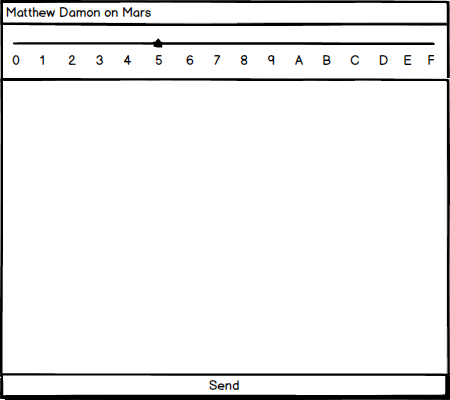
\includegraphics[width=240pt,height=300pt]{/Library/Server/Web/Data/Sites/webserver/PRA/distribute/CSnUsTh4/Assignment4Images/mockup.png}
\caption{An outline of how you frame should appear.}
\label{fig:mockup}
\end{center}
\end{figure}

On this frame, all the items returned from \texttt{getMedia} should be organised into three categories: Films, Music and Unclassified. Films and Music should contain a list of media panes for film and track files, respectively, while Unclassified should contain a list of media panes for those files with no extension (or, conceivably, an unknown extension).

For each film media pane, the appropriate thumbnail should be displayed, while the main text should contain the name of the film \emph{only} and the sub text should contain information about the films year of release and definition, in the form $<$Year Of Release$>$ - $<$Definition$>$ (e.g. 1989 - SD).

For each music media pane, the appropriate thumbnail should be displayed, while the main text should contain the name of the track, and the sub text should contain the name of the artist\footnote{Having the name of the track end in a hyphen, and having the name of the artist start with a hyphen, is undesirable, but permissible.}.

For each unclassified media pane, the appropriate thumbnail should be displayed, while the main text should contain the full (raw) name of the file, and the sub text should simply read `Unclassified'.

In addition, your library frame should offer the following functionality:

\begin{enumerate}

	\item The drop-down box inside Films (Figure \ref{fig:mockup}) should have three options: Title, Release Year and Quality. When one of these options is selected, the media panes inside Films should be re-ordered either by title, their release year, or their quality. Quality, in this context, refers to the number of pixels (e.g. 1080). Title ordering is alphabetic, the release year ordering should start with the \emph{latest} releases furthest to the left of the films category and quality ordering should start with the \emph{highest} quality (i.e. the highest number of pixels) furthest to the left of the films category. Note that title ordering should \textbf{ignore} the leading `The' on any title , meaning that, for example, a film entitled `The City Of Days' would be ordered \emph{before} a film entitled `Playing It Like A Prince'.

	\item The drop-down box inside Music (Figure \ref{fig:mockup}) should have two options: Track Name and Artist, both of which should order the media panes inside Music by track name and artist, respectively. Here, the leading `The' on any track or artist should also be ignored.
	
\end{enumerate}

\subsection{Submitting your work}

\textbf{Ensure your code is correctly annotated with Javadoc comments}, in addition to standard comments.

If, once finished, you wish to submit your work to us for preliminary feedback, you should do so by following the `Additional Support' steps from Step 3.2 onwards (i.e. direct contact), in order to avoid sharing your solution with your peers unnecessarily.

If you are happy with your solution, then you should both submit \emph{identical} copies of it to KEATS, adhering to all the submission rules given in the Q\&A document referenced at the beginning of this project brief. Nothing should differ between the submissions, especially the ordering of the names in the top-level package (i.e. $<$\emph{partnerApartnerB}$>$ should be the order adopted by \textbf{both} students).

The folder you compress for submission should be your top-level package, or the first folder inside your project source. For this assignment, the top-level folder is $<$\emph{partnerApartnerB}$>$. Compress this folder directly, so that the file you submit is of the form $<$\emph{partnerApartnerB}$>$.\\ $<$compression\_extension$>$ (e.g. steffenmartin.zip). Do not include anything else in your submission except folders pertaining to your packages, and your raw Java source files. Submissions with extraneous folders (e.g. `src' or `bin' folders from an IDE, folders pertaining to version control software etc.) will be penalised.

\end{document}
